\chapter{Diseño}
\label{cap:capitulo4}

Tras haber puesto en contexto todo lo anterior, en este capítulo se expondrá, de forma detallada, el proceso seguido para conseguir que un dron detecte y navegue hacia una señal \ac{RF}.\\

Además, se mostrará el desarrollo de una aplicación responsiva, que simula el comportamiento de una señal (en un espacio libre de obstáculos), basada en la aproximación de Friis.\\

Por último, se buscará determinar cuál de los métodos empleados es mejor y por qué, a través de diversas métricas comparativas que se expondrán en detalle posteriormente.\\

\section{Preparación del entorno}
\label{sec:preparacion_del_entorno}

Lo primero que se debía conseguir, era un entorno de simulación compatible con \ac{ROS}, así como un sistema de control de versiones, que nos permitiera mantener la trazabilidad y los backups a mano. Por ello, se estableció un repositorio común en GitHub y se usó el paquete de herramientas dispuesto por \textbf{JdeRobot}.

\subsection{JdeRobot - drones}
\label{subsec:jderobot_drones}

Gracias a esta plataforma, se pudieron obtener los modelos y los módulos necesarios para simular en Gazebo 11 el desempeño de un cuadracóptero, provisto de un sistema autopilot PX4.\\
\newpage
El modelo usado es el \textbf{3DR Iris simulado}, con un plugin de una cámara frontal. Este dispositivo utiliza MAVROS para realizar la comunicación, lo que nos permite enviar y recibir mesajes ROS compatibles con el protocolo de comunicaciones típico de estas aeronaves, MAVLink.\\

\begin{figure} [H]
	\begin{center}
	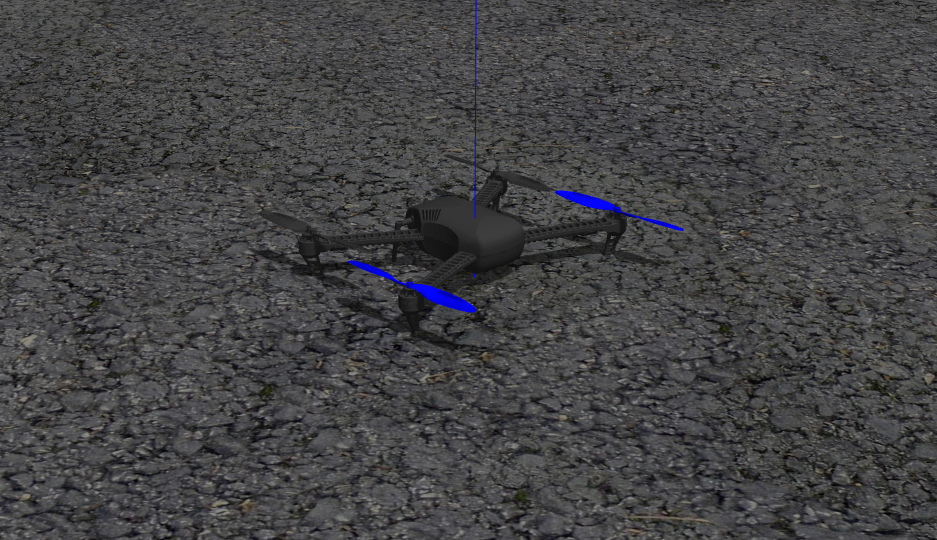
\includegraphics[height=4cm]{imagenes/cap4/1_px4_drone_gz.png}
	\end{center}
	\caption[3DR Iris simulado]{3DR Iris simulado}
	\label{fig:3dr_iris}
\end{figure}

\subsection{Teleoperador}
\label{subsec:teleoperador}

Ya propiamente hablando de resolver el problema planteado, la primera aproximación propuesta fue hacer una interfaz gráfica simple, que permitiera enviar órdenes a la aeronave.\\

Para ello, inicialmente se debía conseguir enviar mensajes de forma programática. Por tanto, se diseñó un \textbf{script controlador} encargado de la comunicación directa con el \textbf{controlador de la aeronave}, para enviar y recibir diversos datos vía MAVROS. De igual modo, se debían satisfacer una serie de requisitos que aseguraran el correcto funcionamiento del sistema:

\begin{enumerate}
	\item La comunicación debe darse a \textbf{más de 2Hz}, para evitar cambios indeseados en el funcionamiento interno del controlador PX4 (de la aeronave).

	\item Antes de realizar cualquier comunicación, \textbf{debe asegurarse que el estado es \emph{``connected''}}, lo que significa que el dron esta armado y en modo \emph{OFFBOARD} (nuestra aeronave posee 7 modos distintos, \emph{HOLD}, que mantiene la posición, \emph{RETURN}, que vuelve al punto de despegue, \emph{MISSION}, que permite cargar rutas programadas con anterioridad, \emph{TAKEOFF}, habilita el despegue, \emph{LAND}, habilita el aterrizaje, \emph{FOLLOW ME}, que permite seguir objetivos, y \emph{OFFBOARD}, que permite comandar al dron sin necesidad de GPS, lo que es útil de cara al desarrollo de aplicaciones robóticas) \cite{flight-modes}.
	
    \item Una vez esta conectado, se deben \textbf{enviar datos} (velocidades en nuestro caso) al controlador PX4, con el fin de \textbf{evitar el cierre de la conexión}. Estos datos carecen de utilidad más que la de asegurar dicha conectividad.
    
    \item Por último, y antes de enviar cualquier posición, velocidad o comando (distintos modos de actuación), se debe comprobar siempre que el \textbf{modo activo} es \emph{OFFBOARD} y que el dron esta \textbf{armado} (listo para volar). En caso contrario, se debe solicitar al controlador, mediante servicios, dichas especificaciones.
\end{enumerate}

Por tanto, con todo esto funcionando de forma correcta, la manera de generar comportamientos en el dron en sí, es mediante \emph{topics}. Concretamente, los que genera MAVROS automáticamente cuando se lanza todo el sistema. Tal y como se comentó en apartados previos, estos \emph{topics} sólo admiten mensajes \ac{ROS}, lo que encapsula el mensaje real transmitido al controlador PX4, que solo es compatible con MAVLINK.\\

En nuestro caso, enviaremos posiciones (PoseStamped), velocidades (Twist) y comandos (sevicios formados por mensajes personalizados, creados por MAVROS, con formato \ac{ROS}). Esto, nos permitirá conectar el resto de aplicaciones con el script controlador, mediante \emph{topics} comunes, de forma que se encargue de enviar la acción final al dron, mientras el resto de scripts se encarguen de resolver otras tareas.\\

De este modo, inicia el desarrollo propiamente dicho del \textbf{teleoperador}. El teleoperador, se diseñó con el fin de generar comportamientos que se usarían en las fases finales del \ac{TFG}. Sin embargo, en la primera versión, tan solo se buscó construir una interfaz gráfica sencilla, capaz de enviar ordenes usando \ac{ROS} que, en última instancia, llegasen al dron y produjesen diversos comportamientos, tales como \textbf{moverse y girar}, a través de sliders.\\

\begin{figure} [H]
	\begin{center}
	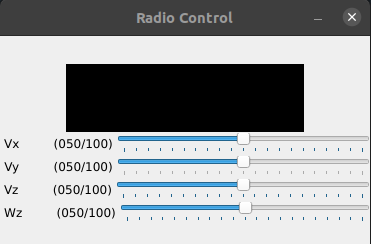
\includegraphics[height=4.5cm]{imagenes/cap4/2_axes_rc.png}
	\end{center}
	\caption[Primera versión del teleoperador]{Primera versión del teleoperador}
	\label{fig:teleoperador_v1}
\end{figure}

En el siguente paso, se buscó programar \textbf{comportamientos predefinidos}, es decir, acciones predeterminadas tales como desplazarse distancias concretas en ciertas direcciones, o girar un número específico de grados en un sentido u otro. Para ello, se diseñó una ampliación sobre la interfaz anterior, en la que se añadió un \textbf{botón por cada acción} concreta desarrollada, además de una \textbf{imagen de la cámara frontal} en directo. Es importante destacar la acción de moverse de distancias específicas, ya que se empleará en los algoritmos posteriores.\\

Finalmente, y continuando con lo anterior, se intentó afinar el comportamiento de las acciones predefinidas, para hacer que el dron se desplazase de celda en celda, concretamente de \textbf{centro en centro}. La idea es que, el dron solo tomará medidas de la señal en posiciones concretas y no en movimiento. Además, se agregaron \textbf{marcadores en \emph{rviz}}, para determinar las celdas visitadas (con colores aleatorios), junto con otro marcador que muestra la trayectoria que sigue la aeronave.\\

\begin{figure} [H]
	\begin{center}
	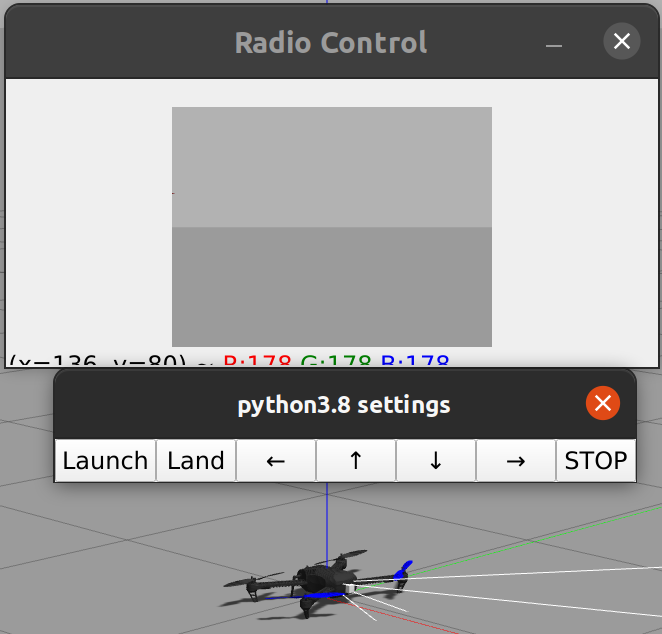
\includegraphics[height=8cm]{imagenes/cap4/3_c2c_gui.png}
	\end{center}
	\caption[Versión final del teleoperador]{Versión final del teleoperador}
	\label{fig:teleoperador_end}
\end{figure}

\newpage
A continuación, se muestra el \emph{``main''} de la aplicación mencionada:\\

\begin{code}[H]
\begin{lstlisting}[language=Python]
if __name__ == '__main__':
    try:
        rospy.init_node(NODENAME, anonymous=True)

        # Msgs
        ## Subscribers
        image_sub = rospy.Subscriber(IMAGE_TOPIC, Image, callback = image_cb)
        current_pos_sub = rospy.Subscriber(LOCAL_POSE_TOPIC, PoseStamped, callback = current_pos_cb)

        ## Publishers
        pos_pub = rospy.Publisher(RADIO_CONTROL_POS_TOPIC, PoseStamped, queue_size=10)
        cmd_pub = rospy.Publisher(RADIO_CONTROL_CMD_TOPIC, Px4Cmd, queue_size=10)

        # -- OPENCV -- #
        cv2.namedWindow(WINDOWNAME)

        # Buttons
        cv2.createButton('Launch', launch_button, None, cv2.QT_PUSH_BUTTON, 1)
        cv2.createButton('Land', land_button, None, cv2.QT_PUSH_BUTTON, 1)
        cv2.createButton('←', left_button, None, cv2.QT_PUSH_BUTTON, 1)
        cv2.createButton('↑', front_button, None, cv2.QT_PUSH_BUTTON, 1)
        cv2.createButton('↓', back_button, None, cv2.QT_PUSH_BUTTON, 1)
        cv2.createButton('→', right_button, None, cv2.QT_PUSH_BUTTON, 1)
        cv2.createButton('STOP', stop_button, None, cv2.QT_PUSH_BUTTON, 1)

        cv2.waitKey(0)
        cv2.destroyAllWindows()
    except rospy.ROSInterruptException:
        pass
\end{lstlisting}
\caption[Main de center to center app]{Main de center to center app}
\label{cod:c2c_app}
\end{code}

Donde, tras inicializar el nodo \ac{ROS}, se definen por un lado los \textbf{suscriptores}, encargados de recibir los datos de la cámara y la posición del dron (usando MAVROS), los \textbf{publicadores}, cuya función es enviar posiciones y/o comandos al script controlador, y por último la \textbf{interfaz gráfica} diseñada con \textbf{OpenCV}, donde se define la ventana y los botones con las diversas acciones predefinidas \footnote{Código completo en \url{https://github.com/RoboticsLabURJC/2022-tfg-cristian-sanchez/blob/main/src/teleop/scripts/c2c_control.py}}.\\

\section{Señales}
\label{sec:signals}

Continuando con el proyecto, entramos en el segundo gran bloque, las señales \ac{RF}. Este apartado, fue especialmente relevante, ya que nos permitió desarrollar una aplicación reactiva, con la meta de generar entornos sobre los que probar soluciones robóticas.\\

Pero, antes de entrar en detalle, conviene familiarizarse con algunos conceptos básicos sobre el procesamiento de señales:

\begin{enumerate}
	\item \textbf{Señal}:
	
    \item \textbf{Dominio temporal}:
    
    \item \textbf{Dominio de la señal}:
    
    \item \textbf{ADC}:
    
    \item \textbf{RSSI}:
    
    \item \textbf{SNR}:

    \item \textbf{Frecuencia}:
    
    \item \textbf{TX}:
    
    \item \textbf{RX}:
\end{enumerate}

Definidos estos términos, nuestro objetivo fue obtener un modelo capaz de calcular la \textbf{propagación de la señal}, es decir, -----.\\

\subsection{Aproximación de Friis}
\label{subsec:friis}

Por ello, se optó por emplear la aproximación de Friis, que nos proporciona una sencilla fórmula sobre la cual modelizar nuestro problema.\\

(insertar fórmula)

Donde cada término significa lo siguiente:

\begin{enumerate}
    \item \textbf{Ganancias}:
    
    \item \textbf{Valor lambda}:
    
    \item \textbf{Distancia (d)}:
    
    \item \textbf{Factor L}: (Insertar tabla)
\end{enumerate}

Además, empleando este método, podemos modelizar las \textbf{pérdidas de una señal} estimadas durante su propagación, a través de la siguiente ecuación:\\

(insertar ecuación path loss)\\

Sin embargo, para nuestro caso no es relevante (aunque se añadió al módulo).\\

\subsection{Módulo python de Friis}
\label{subsec:friis-module}

Una vez realizadas las pruebas iniciales, se buscó compactar todo, en un lugar accesible para cada aplicación que lo necesitase.\\

De este modo, surgió la idea de crear un módulo python que se encargará de modelizar un mapa de señales. Para ello, se diseño una clase cuyo constructor se encarga de recibir por parámetros, las variables implicadas en las ecuaciones de Friis. Además, se debe especificar las dimensiones del mapa y su resolución (que afecta al tamaño de celda).\\

Básicamente, primero se crea un objeto de la clase Friis donde se especifican las características de la señal y el mapa, el cual genera un mapa sin información. Luego, se selecciona el tipo de modelo que se quiera usar (propagación o pérdidas, este último no está testeado), pasando las coordenadas de la señal por parámetros, el cual retornará el mapa relleno con los valores asociados a las ecuaciones de Friis. A continuación se muestra un ejemplo de uso:

\begin{code}[H]
    \begin{lstlisting}[language=Python]

    #! /usr/bin/env python    
    import friss as fr

    if __name__ == '__main__':
        friis_object = fr.Friss(power_tras=10.0, 
                                gain_tras=1.5, 
                                gain_recv=2.0,
                                freq=fr.FREQ_WIFI, 
                                losses_factor=1.0, 
                                losses_path=2.0,
                                world_sz=(10,10), 
                                resolution=1.0)

        signal_map = friis_object.model_power_signal(origin=(5,3))

\end{lstlisting}
\caption[Main de center to center app]{Main de center to center app}
\label{cod:c2c_app}
\end{code}

En este código, se puede ver que se está generando un mapa 10x10 con resolución 1 (es decir, cada celdilla es de 1x1), de una señal WIFI, donde el transmisor emite a 10 W, con una ganancia de 1.5, el receptor posee una ganancia de 2, un factor de pérdidas (L) de 1, es decir, sin pérdidas, y por último, el exponente n (\emph{path-loss exponent (PLE)}) con un valor de 2, que representa el espacio vacío. Luego se genera el mapa de propagación de la señal, indicando que la fuente se encuentra en las coordenadas (5,3).\\

Sin embargo, este módulo posee otras funcionalidades útiles para trabajar con él. Como son:

\begin{enumerate}
    \item \textbf{\emph{reset\_world}}: modifica el mapa que hubiera, estableciendo todos sus valores a cero.
    
    \item \textbf{\emph{get\_world\_sz}}: retorna las dimensiones del mapa.
    
    \item \textbf{\emph{set\_values}}: modifica las características de la señal simulada.
\end{enumerate}

Recordar que aunque se modifiquen los parámetros, se debe modelar de nuevo el mapa para ver los resultados.\\

Por último, se busco extender la funcionalidad del módulo, de manera que fuera posible incluir obstáculos en el mapa. La idea era crear un método capaz de posicionar obstáculos en el mapa de la señal, y simular su efecto en la señal.\\

Para ello, se buscó trazar proyecciones desde la señal hasta los bordes del obstáculo, de forma que se generase un polígono con los bordes del mapa. Posteriormente, se revisó que puntos se encontraban dentro del polígono (que no fueran propiamente parte del obstáculo), a través de un algoritmo basado en el número de intersecciones del punto con el perímetro del polígono, trazando una línea horizontal y hacia la derecha. CITAAAAAAAAR!!!. Por último, para cada punto dentro del polígono se le aplicó un factor de pérdida al valor almacenado de la señal, de manera que se simulase el efecto del obstáculo.\\

(imagenes de los obstáculos)\\

La idea fue abrir puertas a nuevos entornos más complejos y realistas, sobre los que poder probar diversas soluciones, en nuestro caso, para testear el efecto de un muro en el camino del dron a la señal.

(código ejemplo obstáculos)\\

\subsection{Aplicación de Friis}
\label{subsec:friis-app}

La última sección relacionada con las señales se centro en integrar el módulo previo, en una interfaz gráfica amigable para el usuario. La idea era estudiar, en tiempo real, como evolucionaba la señal cuando alguno de sus parametros, en la ecuación de Friis, era modificado.\\

Para llevarlo a cabo, se empleó la librería \textbf{matplotlib}, debido a la enorme cantidad de herramientas de las que dispone, así como de su sencillez a la hora de crear nuevas aplicaciones. Funciona de manera que se generan eventos que son gestionados en \emph{``callbacks''}, es decir, se generan bucles asociados a dichos eventos, que reaccionan a cambios en la interfaz generada. En nuestro caso, la estructura base consta de una figura, sobre la que se agregan todos los elementos, entre los que encontramos los mapas de calor o \emph{``heatmap''} en forma de plots, las barras de acción o \emph{``sliders''}, botones, entre otros elementos que se explicarán más adelante.\\

Inicialmente, se optó por representar un mapa de calor con una barra de color asociada a los distintos valores de la señal. Además, se integraron sliders correspondientes a cada valor presente en la ecuación de Friis, tal y como se muestra a continuación:\\

(imagen app inicial)\\

El problema fue, que al actualizar los valores, también lo hacía la representación, por lo que no se apreciaba el efecto de los cambios en el plot. Por ello, se agregaron dos mapas de calor, uno con el máximo y el mínimo fijados a mano (donde sí se aprecian los cambios), y el anterior mencionado. Para elegir cual usar, se agregó una casilla marcable. Además, se incluyeron dos variables relevantes a la hora de modelar, el \textbf{tamaño del mapa} y la \textbf{resolución}, manejadas a través de \emph{``sliders''}, los cuales a su vez se activan al pulsar un botón de \textbf{SET}, que recarga la interfaz. Además, se ajustó los saltos de valores para que fueran coherentes en el resto de barras de acción, tal y como se puede apreciar a continuación:\\

(imagen app final)\\

\section{Integración conjunta}
\label{sec:integration}

ToDo...